% Generated by Sphinx.
\def\sphinxdocclass{report}
\documentclass[letterpaper,10pt,english]{sphinxmanual}
\usepackage[utf8]{inputenc}
\DeclareUnicodeCharacter{00A0}{\nobreakspace}
\usepackage{cmap}
\usepackage[T1]{fontenc}
\usepackage{babel}
\usepackage{times}
\usepackage[Bjarne]{fncychap}
\usepackage{longtable}
\usepackage{sphinx}
\usepackage{multirow}

\addto\captionsenglish{\renewcommand{\figurename}{Fig. }}
\addto\captionsenglish{\renewcommand{\tablename}{Table }}
\floatname{literal-block}{Listing }



\title{Social Media Mining For Wheater Data Documentation}
\date{September 02, 2015}
\release{0.1}
\author{Dominic Looser}
\newcommand{\sphinxlogo}{}
\renewcommand{\releasename}{Release}
\makeindex

\makeatletter
\def\PYG@reset{\let\PYG@it=\relax \let\PYG@bf=\relax%
    \let\PYG@ul=\relax \let\PYG@tc=\relax%
    \let\PYG@bc=\relax \let\PYG@ff=\relax}
\def\PYG@tok#1{\csname PYG@tok@#1\endcsname}
\def\PYG@toks#1+{\ifx\relax#1\empty\else%
    \PYG@tok{#1}\expandafter\PYG@toks\fi}
\def\PYG@do#1{\PYG@bc{\PYG@tc{\PYG@ul{%
    \PYG@it{\PYG@bf{\PYG@ff{#1}}}}}}}
\def\PYG#1#2{\PYG@reset\PYG@toks#1+\relax+\PYG@do{#2}}

\expandafter\def\csname PYG@tok@gd\endcsname{\def\PYG@tc##1{\textcolor[rgb]{0.63,0.00,0.00}{##1}}}
\expandafter\def\csname PYG@tok@gu\endcsname{\let\PYG@bf=\textbf\def\PYG@tc##1{\textcolor[rgb]{0.50,0.00,0.50}{##1}}}
\expandafter\def\csname PYG@tok@gt\endcsname{\def\PYG@tc##1{\textcolor[rgb]{0.00,0.27,0.87}{##1}}}
\expandafter\def\csname PYG@tok@gs\endcsname{\let\PYG@bf=\textbf}
\expandafter\def\csname PYG@tok@gr\endcsname{\def\PYG@tc##1{\textcolor[rgb]{1.00,0.00,0.00}{##1}}}
\expandafter\def\csname PYG@tok@cm\endcsname{\let\PYG@it=\textit\def\PYG@tc##1{\textcolor[rgb]{0.25,0.50,0.56}{##1}}}
\expandafter\def\csname PYG@tok@vg\endcsname{\def\PYG@tc##1{\textcolor[rgb]{0.73,0.38,0.84}{##1}}}
\expandafter\def\csname PYG@tok@m\endcsname{\def\PYG@tc##1{\textcolor[rgb]{0.13,0.50,0.31}{##1}}}
\expandafter\def\csname PYG@tok@mh\endcsname{\def\PYG@tc##1{\textcolor[rgb]{0.13,0.50,0.31}{##1}}}
\expandafter\def\csname PYG@tok@cs\endcsname{\def\PYG@tc##1{\textcolor[rgb]{0.25,0.50,0.56}{##1}}\def\PYG@bc##1{\setlength{\fboxsep}{0pt}\colorbox[rgb]{1.00,0.94,0.94}{\strut ##1}}}
\expandafter\def\csname PYG@tok@ge\endcsname{\let\PYG@it=\textit}
\expandafter\def\csname PYG@tok@vc\endcsname{\def\PYG@tc##1{\textcolor[rgb]{0.73,0.38,0.84}{##1}}}
\expandafter\def\csname PYG@tok@il\endcsname{\def\PYG@tc##1{\textcolor[rgb]{0.13,0.50,0.31}{##1}}}
\expandafter\def\csname PYG@tok@go\endcsname{\def\PYG@tc##1{\textcolor[rgb]{0.20,0.20,0.20}{##1}}}
\expandafter\def\csname PYG@tok@cp\endcsname{\def\PYG@tc##1{\textcolor[rgb]{0.00,0.44,0.13}{##1}}}
\expandafter\def\csname PYG@tok@gi\endcsname{\def\PYG@tc##1{\textcolor[rgb]{0.00,0.63,0.00}{##1}}}
\expandafter\def\csname PYG@tok@gh\endcsname{\let\PYG@bf=\textbf\def\PYG@tc##1{\textcolor[rgb]{0.00,0.00,0.50}{##1}}}
\expandafter\def\csname PYG@tok@ni\endcsname{\let\PYG@bf=\textbf\def\PYG@tc##1{\textcolor[rgb]{0.84,0.33,0.22}{##1}}}
\expandafter\def\csname PYG@tok@nl\endcsname{\let\PYG@bf=\textbf\def\PYG@tc##1{\textcolor[rgb]{0.00,0.13,0.44}{##1}}}
\expandafter\def\csname PYG@tok@nn\endcsname{\let\PYG@bf=\textbf\def\PYG@tc##1{\textcolor[rgb]{0.05,0.52,0.71}{##1}}}
\expandafter\def\csname PYG@tok@no\endcsname{\def\PYG@tc##1{\textcolor[rgb]{0.38,0.68,0.84}{##1}}}
\expandafter\def\csname PYG@tok@na\endcsname{\def\PYG@tc##1{\textcolor[rgb]{0.25,0.44,0.63}{##1}}}
\expandafter\def\csname PYG@tok@nb\endcsname{\def\PYG@tc##1{\textcolor[rgb]{0.00,0.44,0.13}{##1}}}
\expandafter\def\csname PYG@tok@nc\endcsname{\let\PYG@bf=\textbf\def\PYG@tc##1{\textcolor[rgb]{0.05,0.52,0.71}{##1}}}
\expandafter\def\csname PYG@tok@nd\endcsname{\let\PYG@bf=\textbf\def\PYG@tc##1{\textcolor[rgb]{0.33,0.33,0.33}{##1}}}
\expandafter\def\csname PYG@tok@ne\endcsname{\def\PYG@tc##1{\textcolor[rgb]{0.00,0.44,0.13}{##1}}}
\expandafter\def\csname PYG@tok@nf\endcsname{\def\PYG@tc##1{\textcolor[rgb]{0.02,0.16,0.49}{##1}}}
\expandafter\def\csname PYG@tok@si\endcsname{\let\PYG@it=\textit\def\PYG@tc##1{\textcolor[rgb]{0.44,0.63,0.82}{##1}}}
\expandafter\def\csname PYG@tok@s2\endcsname{\def\PYG@tc##1{\textcolor[rgb]{0.25,0.44,0.63}{##1}}}
\expandafter\def\csname PYG@tok@vi\endcsname{\def\PYG@tc##1{\textcolor[rgb]{0.73,0.38,0.84}{##1}}}
\expandafter\def\csname PYG@tok@nt\endcsname{\let\PYG@bf=\textbf\def\PYG@tc##1{\textcolor[rgb]{0.02,0.16,0.45}{##1}}}
\expandafter\def\csname PYG@tok@nv\endcsname{\def\PYG@tc##1{\textcolor[rgb]{0.73,0.38,0.84}{##1}}}
\expandafter\def\csname PYG@tok@s1\endcsname{\def\PYG@tc##1{\textcolor[rgb]{0.25,0.44,0.63}{##1}}}
\expandafter\def\csname PYG@tok@gp\endcsname{\let\PYG@bf=\textbf\def\PYG@tc##1{\textcolor[rgb]{0.78,0.36,0.04}{##1}}}
\expandafter\def\csname PYG@tok@sh\endcsname{\def\PYG@tc##1{\textcolor[rgb]{0.25,0.44,0.63}{##1}}}
\expandafter\def\csname PYG@tok@ow\endcsname{\let\PYG@bf=\textbf\def\PYG@tc##1{\textcolor[rgb]{0.00,0.44,0.13}{##1}}}
\expandafter\def\csname PYG@tok@sx\endcsname{\def\PYG@tc##1{\textcolor[rgb]{0.78,0.36,0.04}{##1}}}
\expandafter\def\csname PYG@tok@bp\endcsname{\def\PYG@tc##1{\textcolor[rgb]{0.00,0.44,0.13}{##1}}}
\expandafter\def\csname PYG@tok@c1\endcsname{\let\PYG@it=\textit\def\PYG@tc##1{\textcolor[rgb]{0.25,0.50,0.56}{##1}}}
\expandafter\def\csname PYG@tok@kc\endcsname{\let\PYG@bf=\textbf\def\PYG@tc##1{\textcolor[rgb]{0.00,0.44,0.13}{##1}}}
\expandafter\def\csname PYG@tok@c\endcsname{\let\PYG@it=\textit\def\PYG@tc##1{\textcolor[rgb]{0.25,0.50,0.56}{##1}}}
\expandafter\def\csname PYG@tok@mf\endcsname{\def\PYG@tc##1{\textcolor[rgb]{0.13,0.50,0.31}{##1}}}
\expandafter\def\csname PYG@tok@err\endcsname{\def\PYG@bc##1{\setlength{\fboxsep}{0pt}\fcolorbox[rgb]{1.00,0.00,0.00}{1,1,1}{\strut ##1}}}
\expandafter\def\csname PYG@tok@mb\endcsname{\def\PYG@tc##1{\textcolor[rgb]{0.13,0.50,0.31}{##1}}}
\expandafter\def\csname PYG@tok@ss\endcsname{\def\PYG@tc##1{\textcolor[rgb]{0.32,0.47,0.09}{##1}}}
\expandafter\def\csname PYG@tok@sr\endcsname{\def\PYG@tc##1{\textcolor[rgb]{0.14,0.33,0.53}{##1}}}
\expandafter\def\csname PYG@tok@mo\endcsname{\def\PYG@tc##1{\textcolor[rgb]{0.13,0.50,0.31}{##1}}}
\expandafter\def\csname PYG@tok@kd\endcsname{\let\PYG@bf=\textbf\def\PYG@tc##1{\textcolor[rgb]{0.00,0.44,0.13}{##1}}}
\expandafter\def\csname PYG@tok@mi\endcsname{\def\PYG@tc##1{\textcolor[rgb]{0.13,0.50,0.31}{##1}}}
\expandafter\def\csname PYG@tok@kn\endcsname{\let\PYG@bf=\textbf\def\PYG@tc##1{\textcolor[rgb]{0.00,0.44,0.13}{##1}}}
\expandafter\def\csname PYG@tok@o\endcsname{\def\PYG@tc##1{\textcolor[rgb]{0.40,0.40,0.40}{##1}}}
\expandafter\def\csname PYG@tok@kr\endcsname{\let\PYG@bf=\textbf\def\PYG@tc##1{\textcolor[rgb]{0.00,0.44,0.13}{##1}}}
\expandafter\def\csname PYG@tok@s\endcsname{\def\PYG@tc##1{\textcolor[rgb]{0.25,0.44,0.63}{##1}}}
\expandafter\def\csname PYG@tok@kp\endcsname{\def\PYG@tc##1{\textcolor[rgb]{0.00,0.44,0.13}{##1}}}
\expandafter\def\csname PYG@tok@w\endcsname{\def\PYG@tc##1{\textcolor[rgb]{0.73,0.73,0.73}{##1}}}
\expandafter\def\csname PYG@tok@kt\endcsname{\def\PYG@tc##1{\textcolor[rgb]{0.56,0.13,0.00}{##1}}}
\expandafter\def\csname PYG@tok@sc\endcsname{\def\PYG@tc##1{\textcolor[rgb]{0.25,0.44,0.63}{##1}}}
\expandafter\def\csname PYG@tok@sb\endcsname{\def\PYG@tc##1{\textcolor[rgb]{0.25,0.44,0.63}{##1}}}
\expandafter\def\csname PYG@tok@k\endcsname{\let\PYG@bf=\textbf\def\PYG@tc##1{\textcolor[rgb]{0.00,0.44,0.13}{##1}}}
\expandafter\def\csname PYG@tok@se\endcsname{\let\PYG@bf=\textbf\def\PYG@tc##1{\textcolor[rgb]{0.25,0.44,0.63}{##1}}}
\expandafter\def\csname PYG@tok@sd\endcsname{\let\PYG@it=\textit\def\PYG@tc##1{\textcolor[rgb]{0.25,0.44,0.63}{##1}}}

\def\PYGZbs{\char`\\}
\def\PYGZus{\char`\_}
\def\PYGZob{\char`\{}
\def\PYGZcb{\char`\}}
\def\PYGZca{\char`\^}
\def\PYGZam{\char`\&}
\def\PYGZlt{\char`\<}
\def\PYGZgt{\char`\>}
\def\PYGZsh{\char`\#}
\def\PYGZpc{\char`\%}
\def\PYGZdl{\char`\$}
\def\PYGZhy{\char`\-}
\def\PYGZsq{\char`\'}
\def\PYGZdq{\char`\"}
\def\PYGZti{\char`\~}
% for compatibility with earlier versions
\def\PYGZat{@}
\def\PYGZlb{[}
\def\PYGZrb{]}
\makeatother

\renewcommand\PYGZsq{\textquotesingle}

\begin{document}

\maketitle
\tableofcontents
\phantomsection\label{index::doc}


Contents:


\chapter{Flickr}
\label{flickr:flickr}\label{flickr::doc}\label{flickr:social-media-mining-for-wheater-data}\begin{itemize}
\item {} 
Created by Ludicorp in 2004

\item {} 
Acquired by Yahoo in 2005

\item {} 
6 billion images in 2011 (we)

\item {} 
87 million registred users in 2013 (we)

\item {} 
3.5 million new images daily in 2013 (we)

\item {} 
Written in PHP

\end{itemize}


\section{API}
\label{flickr:api}\begin{itemize}
\item {} 
REST endpoint: \href{https://api.flickr.com/services/rest/}{https://api.flickr.com/services/rest/}

\item {} 
Return formats: XML, JSON, ...

\item {} 
Parameters: method, api\_key, format

\end{itemize}


\subsection{flickr.photos.search}
\label{flickr:flickr-photos-search}
Parameters:
\begin{itemize}
\item {} 
woe\_id: A 32-bit identifier that uniquely represents spatial entities

\item {} 
place\_id: A Flickr place id

\end{itemize}

Response structure:

\begin{DUlineblock}{0em}
\item[] photos \textgreater{} photo
\end{DUlineblock}

\begin{DUlineblock}{0em}
\item[] photos: page, pages, perpage, total
\item[] photo: id, latitude, longitude, place\_id, title, woeid
\end{DUlineblock}


\subsection{flickr.places.getInfo}
\label{flickr:flickr-places-getinfo}
Get informations about a place.
Parameters:
\begin{itemize}
\item {} 
woe\_id

\item {} 
place\_id

\end{itemize}

response structure:

\begin{DUlineblock}{0em}
\item[] rsp \textgreater{} place
\item[] place \textgreater{} country
\item[] country \textgreater{} shapedata
\item[] shapedate \textgreater{} polylines, urls
\item[] polylines \textgreater{} polyline
\item[] urls \textgreater{} shapefile
\end{DUlineblock}

\begin{DUlineblock}{0em}
\item[] rsp: stat
\item[] place: place\_id, woeid, latitutude, longitude, place\_url, place\_type, place\_type\_id, timezone, name, woe\_name, has\_shapedata
\item[] country: place\_id, woeid, latitutde, longitude, place\_url
\item[] shapedata: created, alpha, count\_points, count\_edges, has\_donuthole, is\_donuthole
\end{DUlineblock}


\subsection{flickr.places.find}
\label{flickr:flickr-places-find}
Returns a list of place objects for a given query string.

Parameter: query

Response:
\textbar{} rsp \textgreater{} places
\textbar{} places \textgreater{} place*

\begin{DUlineblock}{0em}
\item[] rsp: stat
\item[] places: query, total
\item[] place: place\_id, woeid, latitude, longitude, place\_url, place\_type
\end{DUlineblock}


\subsection{woe id vs place id}
\label{flickr:woe-id-vs-place-id}
WOE = where on earth


\section{Python Library}
\label{flickr:python-library}
We use the library called flickrapi. Documentation: \href{http://stuvel.eu/media/flickrapi-docs/documentation/}{http://stuvel.eu/media/flickrapi-docs/documentation/}


\chapter{Twitter}
\label{twitter:twitter}\label{twitter::doc}

\section{Misc}
\label{twitter:misc}\begin{itemize}
\item {} 
140 Characters per tweet

\item {} 
1.9 million tweets January 2009 (twitter api: up and running, p.4)

\item {} 
340 milion tweets each day (2012)

\item {} 
launched July 2006

\item {} 
Twitter Inc in San Francisco

\end{itemize}


\section{Api}
\label{twitter:api}\begin{itemize}
\item {} 
rest-api vs. streaming api

\end{itemize}

schema:
\begin{itemize}
\item {} 
text

\item {} 
created\_at

\item {} 
coordinates

\item {} 
place

\item {} \begin{description}
\item[{entities}] \leavevmode\begin{itemize}
\item {} \begin{description}
\item[{hashtags}] \leavevmode\begin{itemize}
\item {} 
text

\end{itemize}

\end{description}

\end{itemize}

\end{description}

\end{itemize}


\subsection{REST-api}
\label{twitter:rest-api}
\href{https://api.twitter.com}{https://api.twitter.com}/\{version\}


\subsubsection{Search}
\label{twitter:search}
The Search API is not complete index of all Tweets, but instead an index of recent Tweets.
At the moment that index includes between 6-9 days of Tweets. (\href{https://dev.twitter.com/rest/public/search}{https://dev.twitter.com/rest/public/search})


\section{Tweepy}
\label{twitter:tweepy}
Python library used to connect to Twitter API through python.
\begin{description}
\item[{Schema Place}] \leavevmode
full\_name

\item[{Schema Status streaming-api:}] \leavevmode
contributors
truncated
text
in\_reply\_to\_status\_id
id
favorite\_count
author
\begin{quote}

User
follow\_request\_sent
profile\_use\_background\_image
\end{quote}
\begin{description}
\item[{\_json}] \leavevmode
follow\_request\_sent
profile\_use\_background\_image
default\_profile\_image
id
verified
profile\_image\_url\_https
profile\_sidebar\_fill\_color

\end{description}

\end{description}


\section{Geolocation}
\label{twitter:geolocation}\begin{itemize}
\item {} 
tweet is geotagged by user

\item {} 
in germany 1\% of tweets are geotagged

\item {} 
Approximately 3-5\% of all tweets are geo-enabled (\href{https://github.com/Ccantey/GeoSearch-Tweepy}{https://github.com/Ccantey/GeoSearch-Tweepy})

\item {} 
induce location from user profile

\item {} 
induce location from tweet text

\end{itemize}


\chapter{Results}
\label{results::doc}\label{results:results}
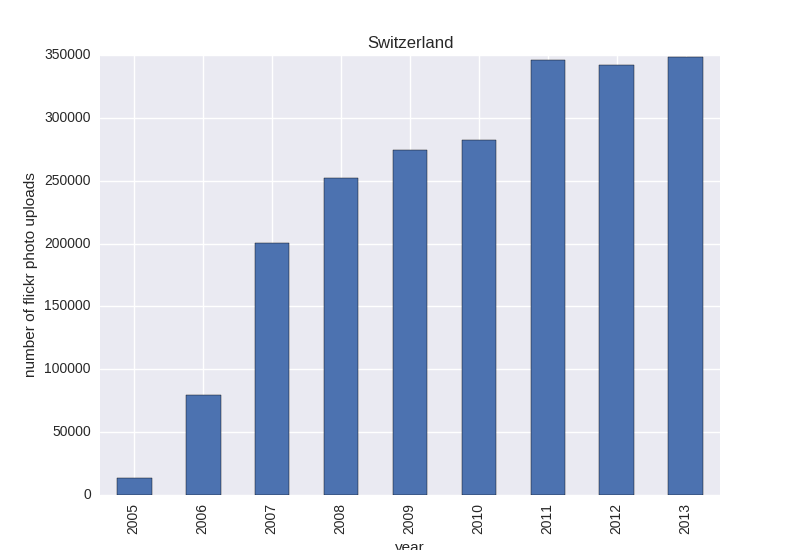
\includegraphics{flickr_switzerland.png}

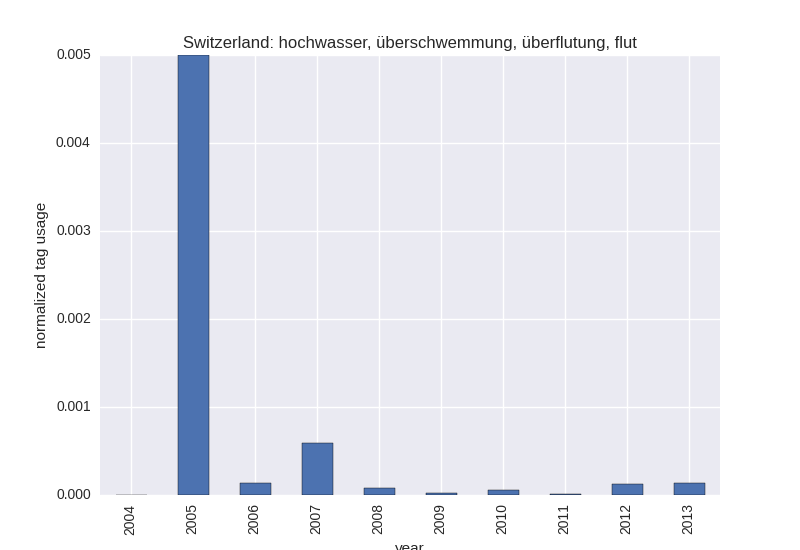
\includegraphics{flickr_flooding_switzerland.png}

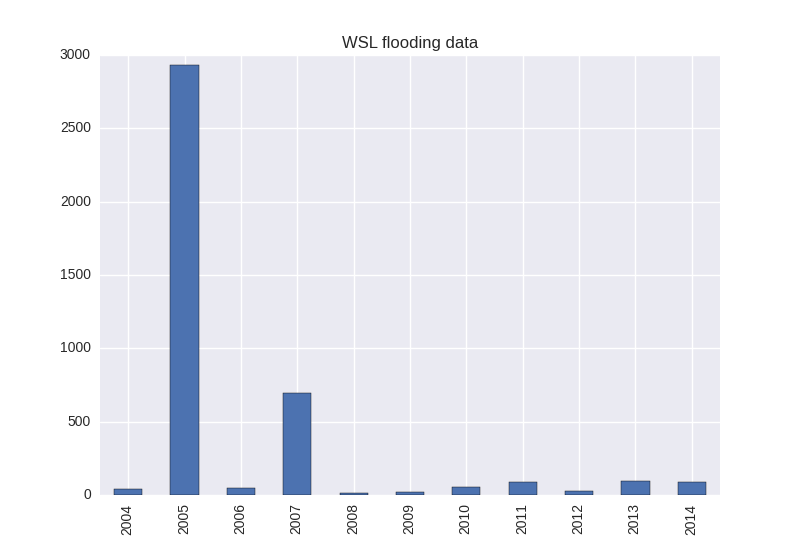
\includegraphics{wsl.png}


\chapter{Codebase}
\label{codebase:codebase}\label{codebase::doc}
All code is based on Python 2.7


\section{Important Libraries}
\label{codebase:important-libraries}\begin{itemize}
\item {} 
Pandas (data analysis)

\item {} 
Matplotlib/Seaborn (plotting)

\item {} 
flickrapi

\item {} 
tweepy

\item {} 
nltk (natural language processing)

\end{itemize}


\chapter{Modules}
\label{modules:modules}\label{modules::doc}

\section{apis package}
\label{apis:apis-package}\label{apis::doc}

\subsection{Submodules}
\label{apis:submodules}

\subsection{apis.facebook\_api module}
\label{apis:apis-facebook-api-module}\label{apis:module-apis.facebook_api}\index{apis.facebook\_api (module)}

\subsection{apis.flickr\_api module}
\label{apis:module-apis.flickr_api}\label{apis:apis-flickr-api-module}\index{apis.flickr\_api (module)}
Classes and functions which abstract over the flickr api.
\index{FlickrQuery (class in apis.flickr\_api)}

\begin{fulllineitems}
\phantomsection\label{apis:apis.flickr_api.FlickrQuery}\pysiglinewithargsret{\strong{class }\code{apis.flickr\_api.}\bfcode{FlickrQuery}}{\emph{tags=None}, \emph{woe\_id=None}, \emph{year=None}, \emph{only\_geotagged=False}}{}
Bases: {\hyperref[apis:apis.Query]{\emph{\code{apis.Query}}}}

\end{fulllineitems}

\index{PhotoCollection (class in apis.flickr\_api)}

\begin{fulllineitems}
\phantomsection\label{apis:apis.flickr_api.PhotoCollection}\pysiglinewithargsret{\strong{class }\code{apis.flickr\_api.}\bfcode{PhotoCollection}}{\emph{iterator}}{}~\index{count\_photos() (apis.flickr\_api.PhotoCollection method)}

\begin{fulllineitems}
\phantomsection\label{apis:apis.flickr_api.PhotoCollection.count_photos}\pysiglinewithargsret{\bfcode{count\_photos}}{}{}
\end{fulllineitems}

\index{get\_random\_link() (apis.flickr\_api.PhotoCollection method)}

\begin{fulllineitems}
\phantomsection\label{apis:apis.flickr_api.PhotoCollection.get_random_link}\pysiglinewithargsret{\bfcode{get\_random\_link}}{}{}
\end{fulllineitems}

\index{to\_points() (apis.flickr\_api.PhotoCollection method)}

\begin{fulllineitems}
\phantomsection\label{apis:apis.flickr_api.PhotoCollection.to_points}\pysiglinewithargsret{\bfcode{to\_points}}{}{}
\end{fulllineitems}


\end{fulllineitems}

\index{count\_photos() (in module apis.flickr\_api)}

\begin{fulllineitems}
\phantomsection\label{apis:apis.flickr_api.count_photos}\pysiglinewithargsret{\code{apis.flickr\_api.}\bfcode{count\_photos}}{\emph{query}}{}
\end{fulllineitems}

\index{get\_photo\_collection() (in module apis.flickr\_api)}

\begin{fulllineitems}
\phantomsection\label{apis:apis.flickr_api.get_photo_collection}\pysiglinewithargsret{\code{apis.flickr\_api.}\bfcode{get\_photo\_collection}}{\emph{query}, \emph{per\_page=200}}{}
\end{fulllineitems}

\index{get\_points() (in module apis.flickr\_api)}

\begin{fulllineitems}
\phantomsection\label{apis:apis.flickr_api.get_points}\pysiglinewithargsret{\code{apis.flickr\_api.}\bfcode{get\_points}}{\emph{query}, \emph{per\_page=200}}{}
\end{fulllineitems}

\index{print\_places() (in module apis.flickr\_api)}

\begin{fulllineitems}
\phantomsection\label{apis:apis.flickr_api.print_places}\pysiglinewithargsret{\code{apis.flickr\_api.}\bfcode{print\_places}}{\emph{query}}{}
\end{fulllineitems}

\index{retrieve\_place\_name() (in module apis.flickr\_api)}

\begin{fulllineitems}
\phantomsection\label{apis:apis.flickr_api.retrieve_place_name}\pysiglinewithargsret{\code{apis.flickr\_api.}\bfcode{retrieve\_place\_name}}{\emph{woe\_id}}{}
\end{fulllineitems}



\subsection{apis.instagram\_api module}
\label{apis:apis-instagram-api-module}\label{apis:module-apis.instagram_api}\index{apis.instagram\_api (module)}

\subsection{apis.twitter\_api module}
\label{apis:module-apis.twitter_api}\label{apis:apis-twitter-api-module}\index{apis.twitter\_api (module)}
Defines important classes Tweet, TwitterSearchQuery, and TwitterStreamingQuery. Enable downloading tweets for search queries and to start streaming with filtering according to a given TwitterStreamingQuery.
\index{PrintingListener (class in apis.twitter\_api)}

\begin{fulllineitems}
\phantomsection\label{apis:apis.twitter_api.PrintingListener}\pysigline{\strong{class }\code{apis.twitter\_api.}\bfcode{PrintingListener}}
Bases: {\hyperref[apis:apis.twitter_api.TwitterStreamListener]{\emph{\code{apis.twitter\_api.TwitterStreamListener}}}}
\index{on\_status() (apis.twitter\_api.PrintingListener method)}

\begin{fulllineitems}
\phantomsection\label{apis:apis.twitter_api.PrintingListener.on_status}\pysiglinewithargsret{\bfcode{on\_status}}{\emph{status}}{}
\end{fulllineitems}


\end{fulllineitems}

\index{StoringListener (class in apis.twitter\_api)}

\begin{fulllineitems}
\phantomsection\label{apis:apis.twitter_api.StoringListener}\pysiglinewithargsret{\strong{class }\code{apis.twitter\_api.}\bfcode{StoringListener}}{\emph{status\_handler}}{}
Bases: {\hyperref[apis:apis.twitter_api.TwitterStreamListener]{\emph{\code{apis.twitter\_api.TwitterStreamListener}}}}
\index{on\_connect() (apis.twitter\_api.StoringListener method)}

\begin{fulllineitems}
\phantomsection\label{apis:apis.twitter_api.StoringListener.on_connect}\pysiglinewithargsret{\bfcode{on\_connect}}{}{}
\end{fulllineitems}

\index{on\_status() (apis.twitter\_api.StoringListener method)}

\begin{fulllineitems}
\phantomsection\label{apis:apis.twitter_api.StoringListener.on_status}\pysiglinewithargsret{\bfcode{on\_status}}{\emph{status}}{}
\end{fulllineitems}


\end{fulllineitems}

\index{Tweet (class in apis.twitter\_api)}

\begin{fulllineitems}
\phantomsection\label{apis:apis.twitter_api.Tweet}\pysiglinewithargsret{\strong{class }\code{apis.twitter\_api.}\bfcode{Tweet}}{\emph{status=None}}{}
Bases: \code{object}

\end{fulllineitems}

\index{TwitterSearchQuery (class in apis.twitter\_api)}

\begin{fulllineitems}
\phantomsection\label{apis:apis.twitter_api.TwitterSearchQuery}\pysiglinewithargsret{\strong{class }\code{apis.twitter\_api.}\bfcode{TwitterSearchQuery}}{\emph{place\_id=None}, \emph{date=None}}{}
Bases: {\hyperref[apis:apis.Query]{\emph{\code{apis.Query}}}}

\end{fulllineitems}

\index{TwitterStreamListener (class in apis.twitter\_api)}

\begin{fulllineitems}
\phantomsection\label{apis:apis.twitter_api.TwitterStreamListener}\pysigline{\strong{class }\code{apis.twitter\_api.}\bfcode{TwitterStreamListener}}
Bases: \code{tweepy.streaming.StreamListener}
\index{on\_error() (apis.twitter\_api.TwitterStreamListener method)}

\begin{fulllineitems}
\phantomsection\label{apis:apis.twitter_api.TwitterStreamListener.on_error}\pysiglinewithargsret{\bfcode{on\_error}}{\emph{status\_code}}{}
\end{fulllineitems}


\end{fulllineitems}

\index{TwitterStreamingQuery (class in apis.twitter\_api)}

\begin{fulllineitems}
\phantomsection\label{apis:apis.twitter_api.TwitterStreamingQuery}\pysiglinewithargsret{\strong{class }\code{apis.twitter\_api.}\bfcode{TwitterStreamingQuery}}{\emph{bounding\_box}}{}
Bases: {\hyperref[apis:apis.Query]{\emph{\code{apis.Query}}}}

\end{fulllineitems}

\index{date\_string\_to\_datetime() (in module apis.twitter\_api)}

\begin{fulllineitems}
\phantomsection\label{apis:apis.twitter_api.date_string_to_datetime}\pysiglinewithargsret{\code{apis.twitter\_api.}\bfcode{date\_string\_to\_datetime}}{\emph{date}}{}
\end{fulllineitems}

\index{download\_search\_tweets() (in module apis.twitter\_api)}

\begin{fulllineitems}
\phantomsection\label{apis:apis.twitter_api.download_search_tweets}\pysiglinewithargsret{\code{apis.twitter\_api.}\bfcode{download\_search\_tweets}}{\emph{query}}{}
\end{fulllineitems}

\index{print\_place\_info() (in module apis.twitter\_api)}

\begin{fulllineitems}
\phantomsection\label{apis:apis.twitter_api.print_place_info}\pysiglinewithargsret{\code{apis.twitter\_api.}\bfcode{print\_place\_info}}{\emph{place\_id}}{}
\end{fulllineitems}

\index{print\_places() (in module apis.twitter\_api)}

\begin{fulllineitems}
\phantomsection\label{apis:apis.twitter_api.print_places}\pysiglinewithargsret{\code{apis.twitter\_api.}\bfcode{print\_places}}{\emph{query\_string}}{}
\end{fulllineitems}

\index{start\_streaming() (in module apis.twitter\_api)}

\begin{fulllineitems}
\phantomsection\label{apis:apis.twitter_api.start_streaming}\pysiglinewithargsret{\code{apis.twitter\_api.}\bfcode{start\_streaming}}{\emph{stream\_listener}, \emph{bounding\_box=None}}{}
\end{fulllineitems}



\subsection{Module contents}
\label{apis:module-contents}\label{apis:module-apis}\index{apis (module)}\index{Query (class in apis)}

\begin{fulllineitems}
\phantomsection\label{apis:apis.Query}\pysigline{\strong{class }\code{apis.}\bfcode{Query}}
Bases: \code{object}

\end{fulllineitems}



\section{config module}
\label{config:module-config}\label{config::doc}\label{config:config-module}\index{config (module)}

\section{flickr\_analysis module}
\label{flickr_analysis:flickr-analysis-module}\label{flickr_analysis::doc}\label{flickr_analysis:module-flickr_analysis}\index{flickr\_analysis (module)}\index{compute\_geotag\_usage() (in module flickr\_analysis)}

\begin{fulllineitems}
\phantomsection\label{flickr_analysis:flickr_analysis.compute_geotag_usage}\pysiglinewithargsret{\code{flickr\_analysis.}\bfcode{compute\_geotag\_usage}}{}{}
\end{fulllineitems}

\index{plot\_normalized\_tag\_usage() (in module flickr\_analysis)}

\begin{fulllineitems}
\phantomsection\label{flickr_analysis:flickr_analysis.plot_normalized_tag_usage}\pysiglinewithargsret{\code{flickr\_analysis.}\bfcode{plot\_normalized\_tag\_usage}}{\emph{tags=None}, \emph{woe\_id=None}, \emph{save2docs=False}}{}
\end{fulllineitems}

\index{plot\_photos\_per\_year() (in module flickr\_analysis)}

\begin{fulllineitems}
\phantomsection\label{flickr_analysis:flickr_analysis.plot_photos_per_year}\pysiglinewithargsret{\code{flickr\_analysis.}\bfcode{plot\_photos\_per\_year}}{\emph{woe\_id=None}, \emph{use\_cache=False}, \emph{save2docs=False}}{}
\end{fulllineitems}

\index{plot\_wsl\_flooding\_data() (in module flickr\_analysis)}

\begin{fulllineitems}
\phantomsection\label{flickr_analysis:flickr_analysis.plot_wsl_flooding_data}\pysiglinewithargsret{\code{flickr\_analysis.}\bfcode{plot\_wsl\_flooding\_data}}{}{}
\end{fulllineitems}

\index{save\_map() (in module flickr\_analysis)}

\begin{fulllineitems}
\phantomsection\label{flickr_analysis:flickr_analysis.save_map}\pysiglinewithargsret{\code{flickr\_analysis.}\bfcode{save\_map}}{\emph{queries, use\_cache=False, n\_bins=60, color\_maps={[}\textless{}matplotlib.colors.LinearSegmentedColormap object at 0x7fc04ab55610\textgreater{}, \textless{}matplotlib.colors.LinearSegmentedColormap object at 0x7fc04ab55650\textgreater{}, \textless{}matplotlib.colors.LinearSegmentedColormap object at 0x7fc04ab55690\textgreater{}{]}, mix\_points=False, formats={[}'png'{]}}}{}
\end{fulllineitems}



\section{geo module}
\label{geo:module-geo}\label{geo::doc}\label{geo:geo-module}\index{geo (module)}\index{BoundingBox (class in geo)}

\begin{fulllineitems}
\phantomsection\label{geo:geo.BoundingBox}\pysigline{\strong{class }\code{geo.}\bfcode{BoundingBox}}
Bases: \code{object}

\end{fulllineitems}

\index{Map (class in geo)}

\begin{fulllineitems}
\phantomsection\label{geo:geo.Map}\pysiglinewithargsret{\strong{class }\code{geo.}\bfcode{Map}}{\emph{bounding\_box}, \emph{map\_resolution=\textless{}MapResolution.INTERMEDIATE: 1\textgreater{}}}{}
Bases: \code{object}
\index{draw\_densities() (geo.Map method)}

\begin{fulllineitems}
\phantomsection\label{geo:geo.Map.draw_densities}\pysiglinewithargsret{\bfcode{draw\_densities}}{\emph{points}, \emph{n\_bins}, \emph{color\_map='Blues'}}{}
\end{fulllineitems}

\index{draw\_points() (geo.Map method)}

\begin{fulllineitems}
\phantomsection\label{geo:geo.Map.draw_points}\pysiglinewithargsret{\bfcode{draw\_points}}{\emph{points}}{}
\end{fulllineitems}

\index{save() (geo.Map method)}

\begin{fulllineitems}
\phantomsection\label{geo:geo.Map.save}\pysiglinewithargsret{\bfcode{save}}{\emph{path}, \emph{format='png'}}{}
\end{fulllineitems}

\index{show() (geo.Map method)}

\begin{fulllineitems}
\phantomsection\label{geo:geo.Map.show}\pysiglinewithargsret{\bfcode{show}}{}{}
\end{fulllineitems}


\end{fulllineitems}

\index{MapResolution (class in geo)}

\begin{fulllineitems}
\phantomsection\label{geo:geo.MapResolution}\pysigline{\strong{class }\code{geo.}\bfcode{MapResolution}}
Bases: \code{enum.Enum}

\end{fulllineitems}

\index{Point (class in geo)}

\begin{fulllineitems}
\phantomsection\label{geo:geo.Point}\pysigline{\strong{class }\code{geo.}\bfcode{Point}}
Bases: \code{object}

\end{fulllineitems}



\section{secrets module}
\label{secrets:module-secrets}\label{secrets::doc}\label{secrets:secrets-module}\index{secrets (module)}

\section{store module}
\label{store:store-module}\label{store:module-store}\label{store::doc}\index{store (module)}\index{StoreType (class in store)}

\begin{fulllineitems}
\phantomsection\label{store:store.StoreType}\pysiglinewithargsret{\strong{class }\code{store.}\bfcode{StoreType}}{\emph{directory}}{}
Bases: \code{object}

\end{fulllineitems}

\index{get\_search\_tweets() (in module store)}

\begin{fulllineitems}
\phantomsection\label{store:store.get_search_tweets}\pysiglinewithargsret{\code{store.}\bfcode{get\_search\_tweets}}{\emph{place\_id}, \emph{begin}, \emph{end=None}, \emph{use\_cache=False}}{}
\end{fulllineitems}

\index{read() (in module store)}

\begin{fulllineitems}
\phantomsection\label{store:store.read}\pysiglinewithargsret{\code{store.}\bfcode{read}}{\emph{query}, \emph{store\_type}}{}
\end{fulllineitems}

\index{save() (in module store)}

\begin{fulllineitems}
\phantomsection\label{store:store.save}\pysiglinewithargsret{\code{store.}\bfcode{save}}{\emph{query}, \emph{store\_type}}{}
\end{fulllineitems}



\section{twitter\_analysis module}
\label{twitter_analysis:module-twitter_analysis}\label{twitter_analysis:twitter-analysis-module}\label{twitter_analysis::doc}\index{twitter\_analysis (module)}\index{Topic (class in twitter\_analysis)}

\begin{fulllineitems}
\phantomsection\label{twitter_analysis:twitter_analysis.Topic}\pysiglinewithargsret{\strong{class }\code{twitter\_analysis.}\bfcode{Topic}}{\emph{terms}}{}
Bases: \code{object}

\end{fulllineitems}

\index{contains\_topic() (in module twitter\_analysis)}

\begin{fulllineitems}
\phantomsection\label{twitter_analysis:twitter_analysis.contains_topic}\pysiglinewithargsret{\code{twitter\_analysis.}\bfcode{contains\_topic}}{\emph{tweet}, \emph{topic}}{}
\end{fulllineitems}

\index{plot\_rain\_data() (in module twitter\_analysis)}

\begin{fulllineitems}
\phantomsection\label{twitter_analysis:twitter_analysis.plot_rain_data}\pysiglinewithargsret{\code{twitter\_analysis.}\bfcode{plot\_rain\_data}}{}{}
\end{fulllineitems}

\index{print\_search\_tweet\_counts() (in module twitter\_analysis)}

\begin{fulllineitems}
\phantomsection\label{twitter_analysis:twitter_analysis.print_search_tweet_counts}\pysiglinewithargsret{\code{twitter\_analysis.}\bfcode{print\_search\_tweet\_counts}}{\emph{place\_id=None}, \emph{begin\_date=None}, \emph{end\_date=None}, \emph{use\_cache=False}}{}
\end{fulllineitems}

\index{topic\_distribution() (in module twitter\_analysis)}

\begin{fulllineitems}
\phantomsection\label{twitter_analysis:twitter_analysis.topic_distribution}\pysiglinewithargsret{\code{twitter\_analysis.}\bfcode{topic\_distribution}}{\emph{topic=None}, \emph{place\_id=None}, \emph{begin=None}, \emph{end=None}, \emph{use\_cache=False}}{}
\end{fulllineitems}



\section{utils module}
\label{utils:utils-module}\label{utils:module-utils}\label{utils::doc}\index{utils (module)}\index{Stopwatch (class in utils)}

\begin{fulllineitems}
\phantomsection\label{utils:utils.Stopwatch}\pysigline{\strong{class }\code{utils.}\bfcode{Stopwatch}}
Bases: \code{object}
\index{start() (utils.Stopwatch method)}

\begin{fulllineitems}
\phantomsection\label{utils:utils.Stopwatch.start}\pysiglinewithargsret{\bfcode{start}}{}{}
\end{fulllineitems}


\end{fulllineitems}

\index{measure\_download\_time() (in module utils)}

\begin{fulllineitems}
\phantomsection\label{utils:utils.measure_download_time}\pysiglinewithargsret{\code{utils.}\bfcode{measure\_download\_time}}{\emph{query}, \emph{per\_page}}{}
\end{fulllineitems}

\index{print\_totals() (in module utils)}

\begin{fulllineitems}
\phantomsection\label{utils:utils.print_totals}\pysiglinewithargsret{\code{utils.}\bfcode{print\_totals}}{\emph{queries}}{}
\end{fulllineitems}



\renewcommand{\indexname}{Python Module Index}
\begin{theindex}
\def\bigletter#1{{\Large\sffamily#1}\nopagebreak\vspace{1mm}}
\bigletter{a}
\item {\texttt{apis}}, \pageref{apis:module-apis}
\item {\texttt{apis.facebook\_api}}, \pageref{apis:module-apis.facebook_api}
\item {\texttt{apis.flickr\_api}}, \pageref{apis:module-apis.flickr_api}
\item {\texttt{apis.instagram\_api}}, \pageref{apis:module-apis.instagram_api}
\item {\texttt{apis.twitter\_api}}, \pageref{apis:module-apis.twitter_api}
\indexspace
\bigletter{c}
\item {\texttt{config}}, \pageref{config:module-config}
\indexspace
\bigletter{f}
\item {\texttt{flickr\_analysis}}, \pageref{flickr_analysis:module-flickr_analysis}
\indexspace
\bigletter{g}
\item {\texttt{geo}}, \pageref{geo:module-geo}
\indexspace
\bigletter{s}
\item {\texttt{secrets}}, \pageref{secrets:module-secrets}
\item {\texttt{store}}, \pageref{store:module-store}
\indexspace
\bigletter{t}
\item {\texttt{twitter\_analysis}}, \pageref{twitter_analysis:module-twitter_analysis}
\indexspace
\bigletter{u}
\item {\texttt{utils}}, \pageref{utils:module-utils}
\end{theindex}

\renewcommand{\indexname}{Index}
\printindex
\end{document}
